\documentclass[]{article}
\usepackage{lmodern}
\usepackage{amssymb,amsmath}
\usepackage{ifxetex,ifluatex}
\usepackage{fixltx2e} % provides \textsubscript
\ifnum 0\ifxetex 1\fi\ifluatex 1\fi=0 % if pdftex
  \usepackage[T1]{fontenc}
  \usepackage[utf8]{inputenc}
\else % if luatex or xelatex
  \ifxetex
    \usepackage{mathspec}
  \else
    \usepackage{fontspec}
  \fi
  \defaultfontfeatures{Ligatures=TeX,Scale=MatchLowercase}
\fi
% use upquote if available, for straight quotes in verbatim environments
\IfFileExists{upquote.sty}{\usepackage{upquote}}{}
% use microtype if available
\IfFileExists{microtype.sty}{%
\usepackage{microtype}
\UseMicrotypeSet[protrusion]{basicmath} % disable protrusion for tt fonts
}{}
\usepackage[margin=1in]{geometry}
\usepackage{hyperref}
\hypersetup{unicode=true,
            pdftitle={Exercises},
            pdfauthor={Bruna Wundervald},
            pdfborder={0 0 0},
            breaklinks=true}
\urlstyle{same}  % don't use monospace font for urls
\usepackage{color}
\usepackage{fancyvrb}
\newcommand{\VerbBar}{|}
\newcommand{\VERB}{\Verb[commandchars=\\\{\}]}
\DefineVerbatimEnvironment{Highlighting}{Verbatim}{commandchars=\\\{\}}
% Add ',fontsize=\small' for more characters per line
\usepackage{framed}
\definecolor{shadecolor}{RGB}{248,248,248}
\newenvironment{Shaded}{\begin{snugshade}}{\end{snugshade}}
\newcommand{\AlertTok}[1]{\textcolor[rgb]{0.94,0.16,0.16}{#1}}
\newcommand{\AnnotationTok}[1]{\textcolor[rgb]{0.56,0.35,0.01}{\textbf{\textit{#1}}}}
\newcommand{\AttributeTok}[1]{\textcolor[rgb]{0.77,0.63,0.00}{#1}}
\newcommand{\BaseNTok}[1]{\textcolor[rgb]{0.00,0.00,0.81}{#1}}
\newcommand{\BuiltInTok}[1]{#1}
\newcommand{\CharTok}[1]{\textcolor[rgb]{0.31,0.60,0.02}{#1}}
\newcommand{\CommentTok}[1]{\textcolor[rgb]{0.56,0.35,0.01}{\textit{#1}}}
\newcommand{\CommentVarTok}[1]{\textcolor[rgb]{0.56,0.35,0.01}{\textbf{\textit{#1}}}}
\newcommand{\ConstantTok}[1]{\textcolor[rgb]{0.00,0.00,0.00}{#1}}
\newcommand{\ControlFlowTok}[1]{\textcolor[rgb]{0.13,0.29,0.53}{\textbf{#1}}}
\newcommand{\DataTypeTok}[1]{\textcolor[rgb]{0.13,0.29,0.53}{#1}}
\newcommand{\DecValTok}[1]{\textcolor[rgb]{0.00,0.00,0.81}{#1}}
\newcommand{\DocumentationTok}[1]{\textcolor[rgb]{0.56,0.35,0.01}{\textbf{\textit{#1}}}}
\newcommand{\ErrorTok}[1]{\textcolor[rgb]{0.64,0.00,0.00}{\textbf{#1}}}
\newcommand{\ExtensionTok}[1]{#1}
\newcommand{\FloatTok}[1]{\textcolor[rgb]{0.00,0.00,0.81}{#1}}
\newcommand{\FunctionTok}[1]{\textcolor[rgb]{0.00,0.00,0.00}{#1}}
\newcommand{\ImportTok}[1]{#1}
\newcommand{\InformationTok}[1]{\textcolor[rgb]{0.56,0.35,0.01}{\textbf{\textit{#1}}}}
\newcommand{\KeywordTok}[1]{\textcolor[rgb]{0.13,0.29,0.53}{\textbf{#1}}}
\newcommand{\NormalTok}[1]{#1}
\newcommand{\OperatorTok}[1]{\textcolor[rgb]{0.81,0.36,0.00}{\textbf{#1}}}
\newcommand{\OtherTok}[1]{\textcolor[rgb]{0.56,0.35,0.01}{#1}}
\newcommand{\PreprocessorTok}[1]{\textcolor[rgb]{0.56,0.35,0.01}{\textit{#1}}}
\newcommand{\RegionMarkerTok}[1]{#1}
\newcommand{\SpecialCharTok}[1]{\textcolor[rgb]{0.00,0.00,0.00}{#1}}
\newcommand{\SpecialStringTok}[1]{\textcolor[rgb]{0.31,0.60,0.02}{#1}}
\newcommand{\StringTok}[1]{\textcolor[rgb]{0.31,0.60,0.02}{#1}}
\newcommand{\VariableTok}[1]{\textcolor[rgb]{0.00,0.00,0.00}{#1}}
\newcommand{\VerbatimStringTok}[1]{\textcolor[rgb]{0.31,0.60,0.02}{#1}}
\newcommand{\WarningTok}[1]{\textcolor[rgb]{0.56,0.35,0.01}{\textbf{\textit{#1}}}}
\usepackage{graphicx,grffile}
\makeatletter
\def\maxwidth{\ifdim\Gin@nat@width>\linewidth\linewidth\else\Gin@nat@width\fi}
\def\maxheight{\ifdim\Gin@nat@height>\textheight\textheight\else\Gin@nat@height\fi}
\makeatother
% Scale images if necessary, so that they will not overflow the page
% margins by default, and it is still possible to overwrite the defaults
% using explicit options in \includegraphics[width, height, ...]{}
\setkeys{Gin}{width=\maxwidth,height=\maxheight,keepaspectratio}
\IfFileExists{parskip.sty}{%
\usepackage{parskip}
}{% else
\setlength{\parindent}{0pt}
\setlength{\parskip}{6pt plus 2pt minus 1pt}
}
\setlength{\emergencystretch}{3em}  % prevent overfull lines
\providecommand{\tightlist}{%
  \setlength{\itemsep}{0pt}\setlength{\parskip}{0pt}}
\setcounter{secnumdepth}{0}
% Redefines (sub)paragraphs to behave more like sections
\ifx\paragraph\undefined\else
\let\oldparagraph\paragraph
\renewcommand{\paragraph}[1]{\oldparagraph{#1}\mbox{}}
\fi
\ifx\subparagraph\undefined\else
\let\oldsubparagraph\subparagraph
\renewcommand{\subparagraph}[1]{\oldsubparagraph{#1}\mbox{}}
\fi

%%% Use protect on footnotes to avoid problems with footnotes in titles
\let\rmarkdownfootnote\footnote%
\def\footnote{\protect\rmarkdownfootnote}

%%% Change title format to be more compact
\usepackage{titling}

% Create subtitle command for use in maketitle
\providecommand{\subtitle}[1]{
  \posttitle{
    \begin{center}\large#1\end{center}
    }
}

\setlength{\droptitle}{-2em}

  \title{Exercises}
    \pretitle{\vspace{\droptitle}\centering\huge}
  \posttitle{\par}
    \author{Bruna Wundervald}
    \preauthor{\centering\large\emph}
  \postauthor{\par}
    \date{}
    \predate{}\postdate{}
  

\begin{document}
\maketitle

\textbf{Exercise 2.1} (Preliminary Simulation). Familiarise yourself
with the support provided by \texttt{R} for simple simulation tasks. In
particular:

\begin{enumerate}
\def\labelenumi{\arabic{enumi}.}
\item
  Generate a large sample of \(N(3,7)\) random variables (see
  \texttt{rnorm}); plot a histogram (hist with sensibly-chosen bins) of
  your sample and overlay a normal density upon it (see \texttt{dnorm},
  \texttt{lines}).
\item
  Use sample to simulate the rolling of 1,000 dice; use your sample to
  estimate the average value obtained when rolling a standard die. Show
  how the estimate obtained using n dice behaves for \(n \in [0, 1000]\)
  using a simple plot.
\end{enumerate}

\begin{Shaded}
\begin{Highlighting}[]
\KeywordTok{set.seed}\NormalTok{(}\DecValTok{2019}\NormalTok{)}

\CommentTok{# Normal exercise ------------------------}
\NormalTok{samp <-}\StringTok{ }\KeywordTok{rnorm}\NormalTok{(}\DecValTok{1000}\NormalTok{, }\DataTypeTok{mean =} \DecValTok{3}\NormalTok{, }\DataTypeTok{sd =} \KeywordTok{sqrt}\NormalTok{(}\DecValTok{7}\NormalTok{))}

\KeywordTok{data.frame}\NormalTok{(samp, }
           \DataTypeTok{dens =} \KeywordTok{dnorm}\NormalTok{(samp, }\DataTypeTok{mean =} \DecValTok{3}\NormalTok{, }\DataTypeTok{sd =} \KeywordTok{sqrt}\NormalTok{(}\DecValTok{7}\NormalTok{))) }\OperatorTok\StringTok{ }
\StringTok{  }\KeywordTok{ggplot}\NormalTok{(}\KeywordTok{aes}\NormalTok{(}\DataTypeTok{x =}\NormalTok{ samp)) }\OperatorTok{+}
\StringTok{  }\KeywordTok{geom_histogram}\NormalTok{(}\DataTypeTok{alpha =} \FloatTok{0.2}\NormalTok{, }
                 \DataTypeTok{fill =} \StringTok{"tomato"}\NormalTok{, }\DataTypeTok{stat =} \StringTok{"density"}\NormalTok{) }\OperatorTok{+}
\StringTok{  }\KeywordTok{geom_line}\NormalTok{(}\KeywordTok{aes}\NormalTok{(}\DataTypeTok{x =}\NormalTok{ samp, }\DataTypeTok{y =}\NormalTok{ dens)) }\OperatorTok{+}
\StringTok{  }\KeywordTok{xlim}\NormalTok{(}\DecValTok{3} \OperatorTok{-}\StringTok{ }\DecValTok{4}\OperatorTok{*}\KeywordTok{sqrt}\NormalTok{(}\DecValTok{7}\NormalTok{), }\DecValTok{3} \OperatorTok{+}\StringTok{ }\DecValTok{4}\OperatorTok{*}\KeywordTok{sqrt}\NormalTok{(}\DecValTok{7}\NormalTok{)) }\OperatorTok{+}
\StringTok{  }\KeywordTok{labs}\NormalTok{(}\DataTypeTok{x =} \StringTok{"Sampled values"}\NormalTok{, }\DataTypeTok{y =} \StringTok{"Density"}\NormalTok{) }\OperatorTok{+}
\StringTok{  }\KeywordTok{theme_bw}\NormalTok{()}
\end{Highlighting}
\end{Shaded}

\begin{center}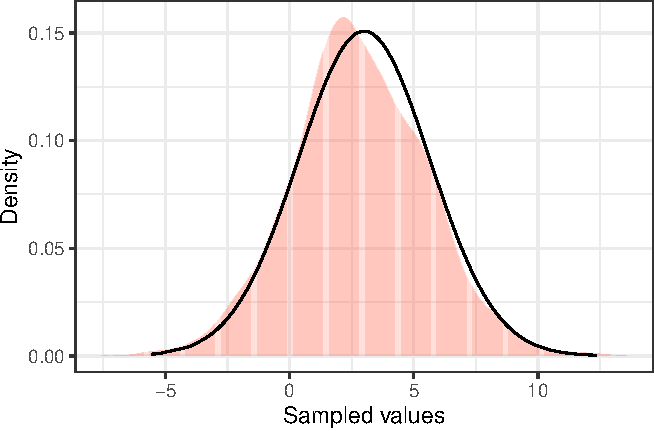
\includegraphics{exercises_files/figure-latex/unnamed-chunk-1-1} \end{center}

\begin{Shaded}
\begin{Highlighting}[]
\CommentTok{# Rolling dices exercise -----------------}
\NormalTok{dice <-}\StringTok{ }\DecValTok{1000}
\NormalTok{vals <-}\StringTok{ }\DecValTok{1}\OperatorTok{:}\DecValTok{6}
\NormalTok{reps <-}\StringTok{ }\KeywordTok{replicate}\NormalTok{(}\DataTypeTok{n =}\NormalTok{ dice, }\KeywordTok{sample}\NormalTok{(vals, }\DataTypeTok{size =} \DecValTok{1}\NormalTok{))}

\KeywordTok{data.frame}\NormalTok{(reps, }
           \DataTypeTok{n =} \DecValTok{1}\OperatorTok{:}\NormalTok{dice,}
           \DataTypeTok{sum =} \KeywordTok{cumsum}\NormalTok{(reps)) }\OperatorTok\StringTok{ }
\StringTok{  }\KeywordTok{mutate}\NormalTok{(}\DataTypeTok{mu_hat =}\NormalTok{ sum}\OperatorTok{/}\NormalTok{n) }\OperatorTok\StringTok{ }
\StringTok{  }\KeywordTok{ggplot}\NormalTok{(}\KeywordTok{aes}\NormalTok{(}\DataTypeTok{x =}\NormalTok{ n, }\DataTypeTok{y =}\NormalTok{ mu_hat)) }\OperatorTok{+}
\StringTok{  }\KeywordTok{geom_hline}\NormalTok{(}\DataTypeTok{yintercept =} \KeywordTok{mean}\NormalTok{(reps)) }\OperatorTok{+}
\StringTok{  }\KeywordTok{geom_point}\NormalTok{(}\DataTypeTok{alpha =} \FloatTok{0.2}\NormalTok{, }
             \DataTypeTok{colour =} \StringTok{"tomato"}\NormalTok{) }\OperatorTok{+}
\StringTok{  }\KeywordTok{labs}\NormalTok{(}\DataTypeTok{x =} \StringTok{"Number of dice rolled"}\NormalTok{, }
       \DataTypeTok{y =} \KeywordTok{expression}\NormalTok{(}\StringTok{"Current estimated "}\OperatorTok{~}\NormalTok{mu)) }\OperatorTok{+}
\StringTok{  }\KeywordTok{theme_bw}\NormalTok{()}
\end{Highlighting}
\end{Shaded}

\begin{center}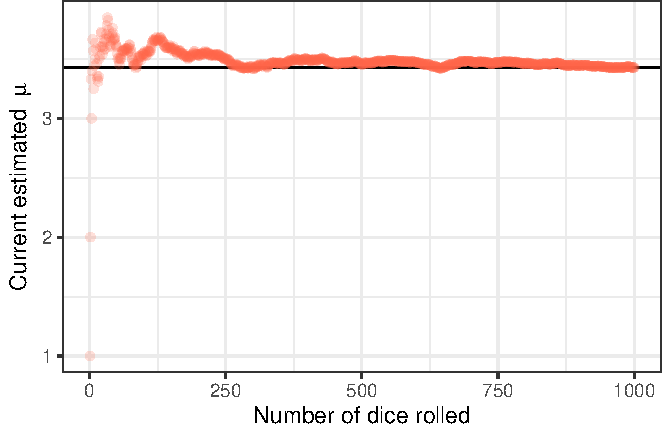
\includegraphics{exercises_files/figure-latex/unnamed-chunk-1-2} \end{center}

\textbf{Exercise 2.2} (Towards Bootstrap Methods). Imagine that you have
a sample of 1,000 values from a population of unknown distribution (for
our purposes, you can obtain such a sample using \texttt{rnorm} as in
the previous question and pretending that the distribution is unknown).

\begin{enumerate}
\def\labelenumi{\arabic{enumi}.}
\tightlist
\item
  Write code to repeat the following 1,000 times:
\end{enumerate}

\begin{enumerate}
\def\labelenumi{(\alph{enumi})}
\tightlist
\item
  Sample 1,000 times with replacement from the original sample to obtain
  1,000 resampled sets of values.
\item
  Compute the sample mean of your resampled set.
\end{enumerate}

\begin{Shaded}
\begin{Highlighting}[]
\NormalTok{samps <-}\StringTok{ }\KeywordTok{map}\NormalTok{(}\DecValTok{1}\OperatorTok{:}\DecValTok{1000}\NormalTok{,}
             \OperatorTok{~}\NormalTok{\{}\KeywordTok{sample}\NormalTok{(samp, }\DataTypeTok{size =} \KeywordTok{length}\NormalTok{(samp),}
                      \DataTypeTok{replace =} \OtherTok{TRUE}\NormalTok{)\}) }\OperatorTok\StringTok{ }
\StringTok{  }\KeywordTok{unlist}\NormalTok{()}


\NormalTok{df <-}\StringTok{ }\KeywordTok{data.frame}\NormalTok{(}\DataTypeTok{samps =}\NormalTok{ samps, }
           \DataTypeTok{ind =} \KeywordTok{rep}\NormalTok{(}\DecValTok{1}\OperatorTok{:}\DecValTok{1000}\NormalTok{, }\DataTypeTok{each =} \KeywordTok{length}\NormalTok{(samp)))}

\NormalTok{df }\OperatorTok\StringTok{ }
\StringTok{  }\KeywordTok{group_by}\NormalTok{(ind) }\OperatorTok\StringTok{ }
\StringTok{  }\KeywordTok{summarise}\NormalTok{(}\DataTypeTok{mu_hat =} \KeywordTok{mean}\NormalTok{(samps)) }\OperatorTok\StringTok{ }
\StringTok{  }\CommentTok{#mutate(dens = dnorm(mu_hat, mean = 3, sd = sqrt(7))) %>% }
\StringTok{  }\KeywordTok{ggplot}\NormalTok{(}\KeywordTok{aes}\NormalTok{(}\DataTypeTok{x =}\NormalTok{ ind, }\DataTypeTok{y =}\NormalTok{ mu_hat)) }\OperatorTok{+}
\StringTok{  }\KeywordTok{geom_hline}\NormalTok{(}\DataTypeTok{yintercept =} \KeywordTok{mean}\NormalTok{(samps)) }\OperatorTok{+}
\StringTok{  }\KeywordTok{geom_point}\NormalTok{(}\DataTypeTok{alpha =} \FloatTok{0.2}\NormalTok{, }
             \DataTypeTok{colour =} \StringTok{"tomato"}\NormalTok{) }\OperatorTok{+}
\StringTok{  }\CommentTok{#geom_line(aes(x = dens, y = mu_hat)) +}
\StringTok{  }\KeywordTok{labs}\NormalTok{(}\DataTypeTok{x =} \StringTok{"Sample number"}\NormalTok{, }
       \DataTypeTok{y =} \KeywordTok{expression}\NormalTok{(}\StringTok{"Estimated "}\OperatorTok{~}\NormalTok{mu)) }\OperatorTok{+}
\StringTok{  }\KeywordTok{theme_bw}\NormalTok{()}
\end{Highlighting}
\end{Shaded}

\begin{center}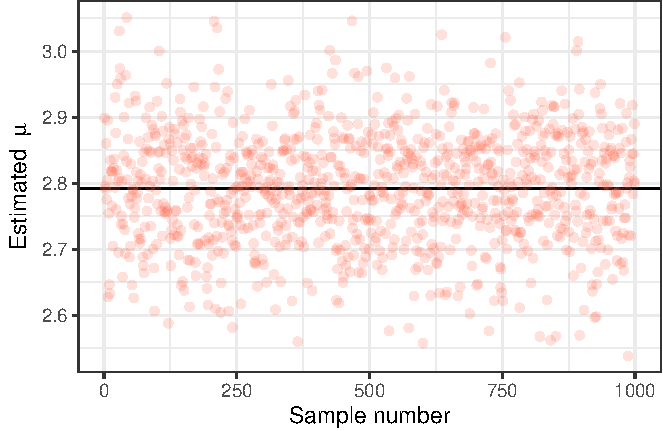
\includegraphics{exercises_files/figure-latex/unnamed-chunk-2-1} \end{center}

\begin{enumerate}
\def\labelenumi{\arabic{enumi}.}
\setcounter{enumi}{1}
\item
  You now have 1,000 sample means for resampled subsets of your data.
  Find the 5th and 95th percentile of this collection of resampled
  means.
\item
  How does this compare with a standard 90\% confidence interval for the
  mean of a sample of size 1,000 from your chosen distribution?
\end{enumerate}

\begin{Shaded}
\begin{Highlighting}[]
\NormalTok{df2 <-}\StringTok{ }\NormalTok{df }\OperatorTok\StringTok{ }
\StringTok{  }\KeywordTok{group_by}\NormalTok{(ind) }\OperatorTok\StringTok{ }
\StringTok{  }\KeywordTok{summarise}\NormalTok{(}\DataTypeTok{perc5 =} \KeywordTok{quantile}\NormalTok{(samps, }\FloatTok{0.05}\NormalTok{),}
            \DataTypeTok{perc95 =} \KeywordTok{quantile}\NormalTok{(samps, }\FloatTok{0.95}\NormalTok{)) }\OperatorTok\StringTok{ }
\StringTok{  }\KeywordTok{gather}\NormalTok{(type, value, }\OperatorTok{-}\NormalTok{ind )  }\OperatorTok\StringTok{ }
\StringTok{  }\KeywordTok{arrange}\NormalTok{(type) }\OperatorTok\StringTok{ }
\StringTok{  }\KeywordTok{mutate}\NormalTok{(}\DataTypeTok{confs =} 
           \KeywordTok{rep}\NormalTok{(}
             \KeywordTok{c}\NormalTok{(}\KeywordTok{mean}\NormalTok{(samp) }\OperatorTok{-}\StringTok{ }\FloatTok{1.96} \OperatorTok{*}\StringTok{ }\KeywordTok{sd}\NormalTok{(samp), }
               \KeywordTok{mean}\NormalTok{(samp) }\OperatorTok{+}\StringTok{ }\FloatTok{1.96} \OperatorTok{*}\StringTok{ }\KeywordTok{sd}\NormalTok{(samp)), }
             \DataTypeTok{each =} \DecValTok{1000}\NormalTok{))}

\NormalTok{df2 }\OperatorTok\StringTok{ }
\KeywordTok{ggplot}\NormalTok{(}\KeywordTok{aes}\NormalTok{(}\DataTypeTok{x =}\NormalTok{ ind, }\DataTypeTok{y =}\NormalTok{ value)) }\OperatorTok{+}
\StringTok{  }\KeywordTok{facet_wrap}\NormalTok{(}\OperatorTok{~}\NormalTok{type, }\DataTypeTok{scales =} \StringTok{"free"}\NormalTok{) }\OperatorTok{+}
\StringTok{  }\KeywordTok{geom_hline}\NormalTok{(}\DataTypeTok{data =}\NormalTok{ df2, }
             \KeywordTok{aes}\NormalTok{(}\DataTypeTok{yintercept =}\NormalTok{ confs)) }\OperatorTok{+}
\StringTok{  }\KeywordTok{geom_point}\NormalTok{(}\DataTypeTok{alpha =} \FloatTok{0.2}\NormalTok{, }
             \DataTypeTok{colour =} \StringTok{"tomato"}\NormalTok{) }\OperatorTok{+}
\StringTok{  }\KeywordTok{labs}\NormalTok{(}\DataTypeTok{x =} \StringTok{"Sample number"}\NormalTok{, }
       \DataTypeTok{y =} \StringTok{"Percentiles: 5% and 95%"}\NormalTok{) }\OperatorTok{+}
\StringTok{  }\KeywordTok{theme_bw}\NormalTok{()}
\end{Highlighting}
\end{Shaded}

\begin{center}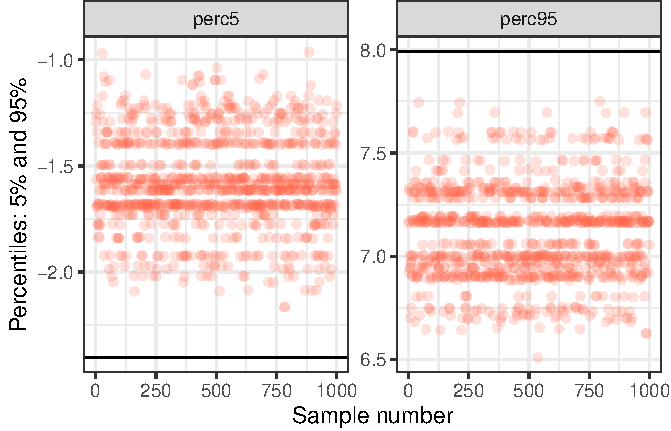
\includegraphics{exercises_files/figure-latex/unnamed-chunk-3-1} \end{center}

\begin{enumerate}
\def\labelenumi{\arabic{enumi}.}
\setcounter{enumi}{3}
\item
  Repeat the above using the median rather than mean.
\item
  Why might this be a useful technique? Note that we haven't done
  anything to justify the approach yet.
\end{enumerate}

\begin{Shaded}
\begin{Highlighting}[]
\NormalTok{df }\OperatorTok\StringTok{ }
\StringTok{  }\KeywordTok{group_by}\NormalTok{(ind) }\OperatorTok\StringTok{ }
\StringTok{  }\KeywordTok{summarise}\NormalTok{(}\DataTypeTok{median_hat =} \KeywordTok{median}\NormalTok{(samps)) }\OperatorTok\StringTok{ }
\StringTok{  }\KeywordTok{ggplot}\NormalTok{(}\KeywordTok{aes}\NormalTok{(}\DataTypeTok{x =}\NormalTok{ ind, }\DataTypeTok{y =}\NormalTok{ median_hat)) }\OperatorTok{+}
\StringTok{  }\KeywordTok{geom_hline}\NormalTok{(}\DataTypeTok{yintercept =} \KeywordTok{median}\NormalTok{(samps)) }\OperatorTok{+}
\StringTok{  }\KeywordTok{geom_point}\NormalTok{(}\DataTypeTok{alpha =} \FloatTok{0.2}\NormalTok{, }
             \DataTypeTok{colour =} \StringTok{"tomato"}\NormalTok{) }\OperatorTok{+}
\StringTok{  }\KeywordTok{labs}\NormalTok{(}\DataTypeTok{x =} \StringTok{"Sample number"}\NormalTok{, }
       \DataTypeTok{y =} \KeywordTok{expression}\NormalTok{(}\StringTok{"Estimated median"}\NormalTok{)) }\OperatorTok{+}
\StringTok{  }\KeywordTok{theme_bw}\NormalTok{()}
\end{Highlighting}
\end{Shaded}

\begin{center}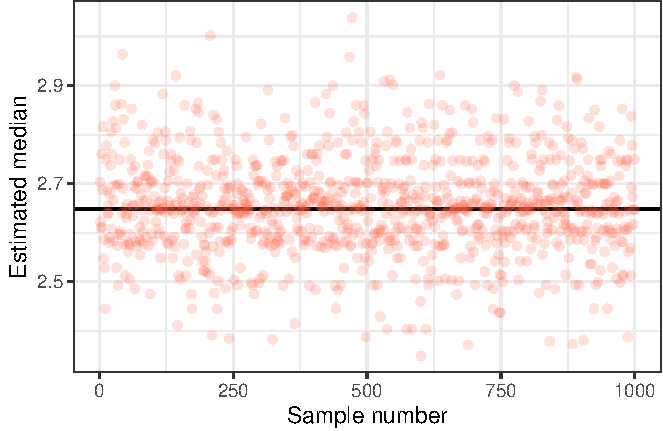
\includegraphics{exercises_files/figure-latex/unnamed-chunk-4-1} \end{center}

\textbf{Exercise 2.3 (Transformation Methods)}. The Box-Muller method
transforms a pair of uniformly- distributed random variables to obtain a
pair of independent standard normal random variates. If

\[U_1, U_2 \sim U[0,1]\]

and

\[ X_1 = \sqrt{-2log(U_1)} cos(2\pi U_2)\]
\[ X_2 = \sqrt{-2log(U_1)} cot(2\pi U_2),\]

then \(X_1, X_2 \sim N(0, 1)\).

\begin{enumerate}
\def\labelenumi{(\alph{enumi})}
\item
  Write a function which takes as arguments two vectors \((U_1, U_2)\)
  of uniformly distributed random variables, and returns the two vectors
  \((X_1, X_2)\) obtained by applying the Box-Muller transform
  elementwise.
\item
  The \texttt{R} function runif provides access to a `pseudo-random
  number generator' (PRNG), which we'll discuss further during the
  module. Generate 10,000 \(U[0,1]\) random variables using this
  function, and transform this vector to two vectors, each of 5,000
  normal random variates.
\item
  Check that the result from (b) is plausibly distributed as pairs of
  independent, standard normal random variables, by creating a scatter
  plot of your data.
\end{enumerate}

\begin{Shaded}
\begin{Highlighting}[]
\NormalTok{u1 <-}\StringTok{ }\KeywordTok{runif}\NormalTok{(}\DecValTok{5000}\NormalTok{)}
\NormalTok{u2 <-}\StringTok{ }\KeywordTok{runif}\NormalTok{(}\DecValTok{5000}\NormalTok{)}

\NormalTok{bm <-}\StringTok{ }\ControlFlowTok{function}\NormalTok{(u1, u2) \{}
\NormalTok{  x1 <-}\StringTok{ }\KeywordTok{sqrt}\NormalTok{(}\OperatorTok{-}\DecValTok{2} \OperatorTok{*}\StringTok{ }\KeywordTok{log}\NormalTok{(u1))}\OperatorTok{*}\KeywordTok{cos}\NormalTok{(}\DecValTok{2}\OperatorTok{*}\NormalTok{pi}\OperatorTok{*}\NormalTok{u2) }
\NormalTok{  x2 <-}\StringTok{ }\KeywordTok{sqrt}\NormalTok{(}\OperatorTok{-}\DecValTok{2} \OperatorTok{*}\StringTok{ }\KeywordTok{log}\NormalTok{(u2))}\OperatorTok{*}\KeywordTok{cos}\NormalTok{(}\DecValTok{2}\OperatorTok{*}\NormalTok{pi}\OperatorTok{*}\NormalTok{u1) }
  \KeywordTok{return}\NormalTok{(}\KeywordTok{data.frame}\NormalTok{(}\DataTypeTok{x1 =}\NormalTok{ x1, }\DataTypeTok{x2 =}\NormalTok{ x2))}
\NormalTok{\}}
  
\NormalTok{x <-}\StringTok{ }\KeywordTok{bm}\NormalTok{(u1, u2) }

\NormalTok{x }\OperatorTok\StringTok{ }
\StringTok{  }\KeywordTok{gather}\NormalTok{(type, value) }\OperatorTok\StringTok{ }
\StringTok{  }\KeywordTok{mutate}\NormalTok{(}\DataTypeTok{dens =} \KeywordTok{dnorm}\NormalTok{(value)) }\OperatorTok\StringTok{ }
\StringTok{  }\KeywordTok{ggplot}\NormalTok{(}\KeywordTok{aes}\NormalTok{(}\DataTypeTok{x =}\NormalTok{ value)) }\OperatorTok{+}
\StringTok{  }\KeywordTok{facet_wrap}\NormalTok{(}\OperatorTok{~}\NormalTok{type) }\OperatorTok{+}
\StringTok{  }\KeywordTok{geom_histogram}\NormalTok{(}\DataTypeTok{alpha =} \FloatTok{0.2}\NormalTok{, }
                 \DataTypeTok{fill =} \StringTok{"tomato"}\NormalTok{, }\DataTypeTok{stat =} \StringTok{"density"}\NormalTok{) }\OperatorTok{+}
\StringTok{  }\KeywordTok{geom_line}\NormalTok{(}\KeywordTok{aes}\NormalTok{(}\DataTypeTok{x =}\NormalTok{ value, }\DataTypeTok{y =}\NormalTok{ dens)) }\OperatorTok{+}
\StringTok{  }\KeywordTok{xlim}\NormalTok{(}\OperatorTok{-}\FloatTok{3.5}\NormalTok{, }\FloatTok{3.5}\NormalTok{) }\OperatorTok{+}
\StringTok{  }\KeywordTok{labs}\NormalTok{(}\DataTypeTok{x =} \StringTok{"New variables"}\NormalTok{, }\DataTypeTok{y =} \StringTok{"Density"}\NormalTok{) }\OperatorTok{+}
\StringTok{  }\KeywordTok{theme_bw}\NormalTok{()}
\end{Highlighting}
\end{Shaded}

\begin{center}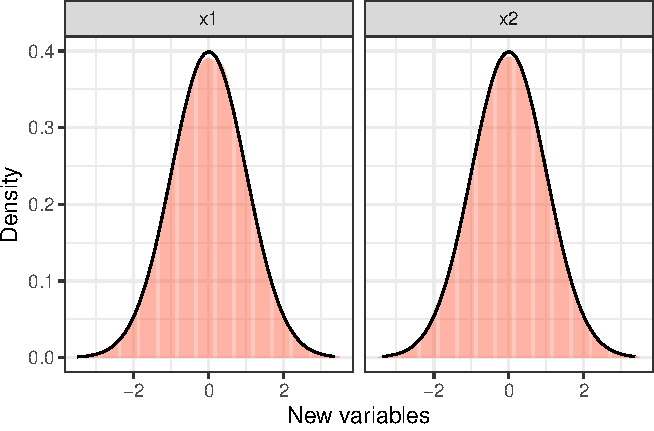
\includegraphics{exercises_files/figure-latex/unnamed-chunk-5-1} \end{center}

\textbf{Exercise 2.4 (Simulating Markov chains)}. Consider a simple
board game in which players take it in turns to move around a circular
board in which an annulus is divided into 40 segments. Players move by
rolling two standard dice and moving their playing piece, clockwise
around the annulus, the number of spaces indicated. For simplicity we'll
neglect the game's other features.

\begin{enumerate}
\def\labelenumi{\arabic{enumi}.}
\tightlist
\item
  All players begin in a common space. Write R code to simulate a
  player's position after three moves of the game and repeat this 1,000
  or so times. Plot a histogram to show the distribution of player
  positions after three moves. Is this consistent with your
  expectations?
\end{enumerate}

\begin{Shaded}
\begin{Highlighting}[]
\NormalTok{numb <-}\StringTok{ }\DecValTok{1}\OperatorTok{:}\DecValTok{40}
\NormalTok{dice <-}\StringTok{  }\DecValTok{2}

\NormalTok{game <-}\StringTok{ }\ControlFlowTok{function}\NormalTok{(samp_player)\{}
  \ControlFlowTok{for}\NormalTok{(i }\ControlFlowTok{in} \DecValTok{1}\OperatorTok{:}\DecValTok{3}\NormalTok{)\{}
\NormalTok{    add <-}\StringTok{ }\KeywordTok{replicate}\NormalTok{(}\DataTypeTok{n =}\NormalTok{ dice, }\KeywordTok{sample}\NormalTok{(vals, }\DataTypeTok{size =} \DecValTok{1}\NormalTok{)) }\OperatorTok\StringTok{ }\KeywordTok{sum}\NormalTok{()}
\NormalTok{    samp_player <-}\StringTok{ }\NormalTok{samp_player }\OperatorTok{+}\StringTok{ }\NormalTok{add}
    \ControlFlowTok{if}\NormalTok{(samp_player }\OperatorTok{>}\StringTok{ }\DecValTok{40}\NormalTok{)\{}
\NormalTok{      samp_player =}\StringTok{ }\NormalTok{samp_player }\OperatorTok{-}\StringTok{ }\DecValTok{40}
\NormalTok{    \}}
\NormalTok{  \}}
  \KeywordTok{return}\NormalTok{(samp_player)}
\NormalTok{\}  }
\NormalTok{game <-}\StringTok{ }\KeywordTok{Vectorize}\NormalTok{(game, }\StringTok{"samp_player"}\NormalTok{)}
  
\CommentTok{#players <- replicate(1000, sample(numb, size = 1))}

\NormalTok{games <-}\StringTok{ }\KeywordTok{data.frame}\NormalTok{(}\DataTypeTok{game =} \KeywordTok{game}\NormalTok{(}\KeywordTok{rep}\NormalTok{(}\DecValTok{1}\NormalTok{, }\DecValTok{1000}\NormalTok{)))}

\NormalTok{games }\OperatorTok\StringTok{ }
\StringTok{  }\KeywordTok{ggplot}\NormalTok{(}\KeywordTok{aes}\NormalTok{(}\DataTypeTok{x =}\NormalTok{ game)) }\OperatorTok{+}
\StringTok{  }\KeywordTok{geom_histogram}\NormalTok{(}\DataTypeTok{alpha =} \FloatTok{0.2}\NormalTok{, }
                 \DataTypeTok{fill =} \StringTok{"tomato"}\NormalTok{,}
                 \DataTypeTok{stat =} \StringTok{"density"}\NormalTok{) }\OperatorTok{+}
\StringTok{  }\KeywordTok{labs}\NormalTok{(}\DataTypeTok{x =} \StringTok{"Results"}\NormalTok{, }\DataTypeTok{y =} \StringTok{"Density"}\NormalTok{) }\OperatorTok{+}
\StringTok{  }\KeywordTok{theme_bw}\NormalTok{()}
\end{Highlighting}
\end{Shaded}

\begin{center}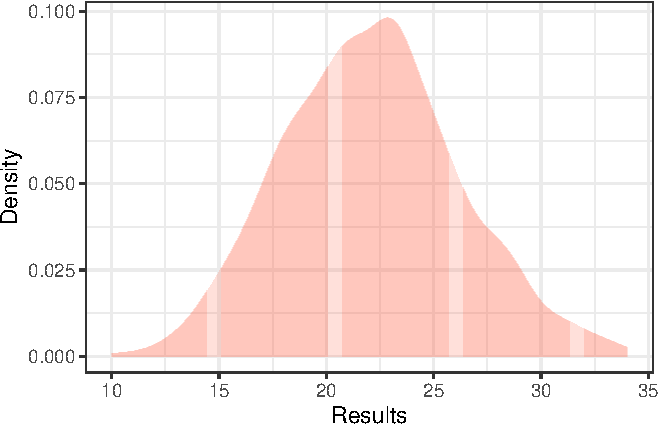
\includegraphics{exercises_files/figure-latex/unnamed-chunk-6-1} \end{center}

\begin{enumerate}
\def\labelenumi{\arabic{enumi}.}
\setcounter{enumi}{1}
\tightlist
\item
  Now modify your code to simulate the sequence of spaces occupied by a
  player over their first 10,000 moves. Plot a histogram to show the
  occupancy of each of the forty spaces during these 10,000 moves. Are
  there any interesting features?
\end{enumerate}

\begin{Shaded}
\begin{Highlighting}[]
\NormalTok{game <-}\StringTok{ }\ControlFlowTok{function}\NormalTok{(samp_player)\{}
\NormalTok{  res <-}\StringTok{ }\KeywordTok{vector}\NormalTok{(}\DataTypeTok{length =} \DecValTok{10000}\NormalTok{)}
\NormalTok{  res[}\DecValTok{1}\NormalTok{] <-}\StringTok{ }\NormalTok{samp_player}
  \ControlFlowTok{for}\NormalTok{(i }\ControlFlowTok{in} \DecValTok{1}\OperatorTok{:}\DecValTok{10000}\NormalTok{)\{}
\NormalTok{    add <-}\StringTok{ }\KeywordTok{replicate}\NormalTok{(}\DataTypeTok{n =}\NormalTok{ dice, }\KeywordTok{sample}\NormalTok{(vals, }\DataTypeTok{size =} \DecValTok{1}\NormalTok{)) }\OperatorTok\StringTok{ }\KeywordTok{sum}\NormalTok{()}
\NormalTok{    res[i}\OperatorTok{+}\DecValTok{1}\NormalTok{] <-}\StringTok{ }\NormalTok{res[i] }\OperatorTok{+}\StringTok{ }\NormalTok{add}
    \ControlFlowTok{if}\NormalTok{(res[i}\OperatorTok{+}\DecValTok{1}\NormalTok{]  }\OperatorTok{>}\StringTok{ }\DecValTok{40}\NormalTok{)\{}
\NormalTok{      res[i}\OperatorTok{+}\DecValTok{1}\NormalTok{]  =}\StringTok{ }\NormalTok{res[i}\OperatorTok{+}\DecValTok{1}\NormalTok{]  }\OperatorTok{-}\StringTok{ }\DecValTok{40}
\NormalTok{    \}}
\NormalTok{  \}}
  \KeywordTok{return}\NormalTok{(res)}
\NormalTok{\}  }

\NormalTok{games <-}\StringTok{ }\KeywordTok{data.frame}\NormalTok{(}\DataTypeTok{game =} \KeywordTok{game}\NormalTok{(}\DecValTok{1}\NormalTok{))}

\NormalTok{games }\OperatorTok\StringTok{ }
\StringTok{  }\KeywordTok{ggplot}\NormalTok{(}\KeywordTok{aes}\NormalTok{(}\DataTypeTok{x =}\NormalTok{ game)) }\OperatorTok{+}
\StringTok{  }\KeywordTok{geom_histogram}\NormalTok{(}\DataTypeTok{alpha =} \FloatTok{0.2}\NormalTok{, }
                 \DataTypeTok{fill =} \StringTok{"tomato"}\NormalTok{,}
                 \DataTypeTok{stat =} \StringTok{"density"}\NormalTok{) }\OperatorTok{+}
\StringTok{  }\KeywordTok{labs}\NormalTok{(}\DataTypeTok{x =} \StringTok{"Results"}\NormalTok{, }\DataTypeTok{y =} \StringTok{"Density"}\NormalTok{) }\OperatorTok{+}
\StringTok{  }\KeywordTok{theme_bw}\NormalTok{()}
\end{Highlighting}
\end{Shaded}

\begin{center}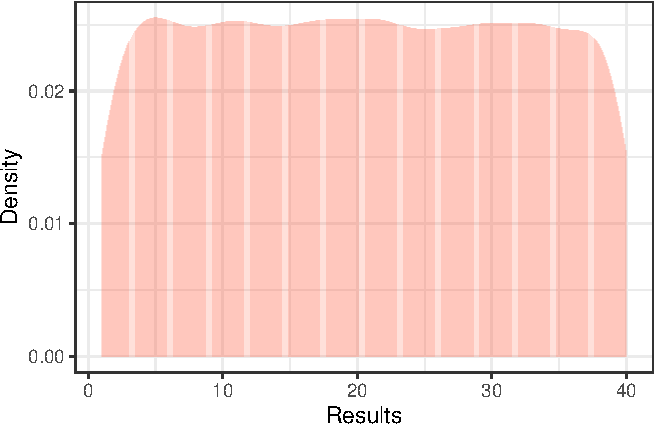
\includegraphics{exercises_files/figure-latex/unnamed-chunk-7-1} \end{center}

\begin{enumerate}
\def\labelenumi{\arabic{enumi}.}
\setcounter{enumi}{2}
\tightlist
\item
  If a player's score increases by 1 every time they land on the first
  space (the starting space), 2 every time they land in the space after
  that and so on up to 40 for landing in the space immediately before
  that space then approximately what would be the long-run average
  number of points per move (use your simulation to obtain an
  approximate answer).
\end{enumerate}

\begin{Shaded}
\begin{Highlighting}[]
\CommentTok{# ?}
\DecValTok{2}\OperatorTok{*}\KeywordTok{mean}\NormalTok{(games}\OperatorTok{$}\NormalTok{game)}
\end{Highlighting}
\end{Shaded}

\begin{verbatim}
## [1] 40.94291
\end{verbatim}

\begin{Shaded}
\begin{Highlighting}[]
\NormalTok{game <-}\StringTok{ }\ControlFlowTok{function}\NormalTok{(samp_player)\{}
\NormalTok{  res <-}\StringTok{ }\KeywordTok{vector}\NormalTok{(}\DataTypeTok{length =} \DecValTok{10000}\NormalTok{)}
\NormalTok{  diff <-}\StringTok{ }\KeywordTok{vector}\NormalTok{(}\DataTypeTok{length =} \DecValTok{10000}\NormalTok{)}
\NormalTok{  res[}\DecValTok{1}\NormalTok{] <-}\StringTok{ }\NormalTok{samp_player}
\NormalTok{  diff[}\DecValTok{1}\NormalTok{] <-}\StringTok{ }\DecValTok{0}
  \ControlFlowTok{for}\NormalTok{(i }\ControlFlowTok{in} \DecValTok{1}\OperatorTok{:}\DecValTok{10000}\NormalTok{)\{}
\NormalTok{    add <-}\StringTok{ }\KeywordTok{replicate}\NormalTok{(}\DataTypeTok{n =}\NormalTok{ dice, }\KeywordTok{sample}\NormalTok{(vals, }\DataTypeTok{size =} \DecValTok{1}\NormalTok{)) }\OperatorTok\StringTok{ }\KeywordTok{sum}\NormalTok{()}
\NormalTok{    res[i}\OperatorTok{+}\DecValTok{1}\NormalTok{] <-}\StringTok{ }\NormalTok{res[i] }\OperatorTok{+}\StringTok{ }\NormalTok{add}
\NormalTok{    diff[i}\OperatorTok{+}\DecValTok{1}\NormalTok{] <-}\StringTok{ }\NormalTok{(res[i] }\OperatorTok{+}\StringTok{ }\NormalTok{add)}\OperatorTok{*}\DecValTok{2} \OperatorTok{-}\StringTok{ }\NormalTok{res[i] }
    \ControlFlowTok{if}\NormalTok{(res[i}\OperatorTok{+}\DecValTok{1}\NormalTok{]  }\OperatorTok{>}\StringTok{ }\DecValTok{40}\NormalTok{)\{}
\NormalTok{      res[i}\OperatorTok{+}\DecValTok{1}\NormalTok{]  =}\StringTok{ }\NormalTok{res[i}\OperatorTok{+}\DecValTok{1}\NormalTok{]  }\OperatorTok{-}\StringTok{ }\DecValTok{40}
\NormalTok{    \}}
\NormalTok{  \}}
  \KeywordTok{return}\NormalTok{(diff)}
\NormalTok{\}  }

\NormalTok{games <-}\StringTok{ }\KeywordTok{data.frame}\NormalTok{(}\DataTypeTok{game =} \KeywordTok{game}\NormalTok{(}\DecValTok{1}\NormalTok{))}
\KeywordTok{mean}\NormalTok{(games}\OperatorTok{$}\NormalTok{game)}
\end{Highlighting}
\end{Shaded}

\begin{verbatim}
## [1] 34.62694
\end{verbatim}

\textbf{Exercise A.1.} What are the maximum likelihood estimators for
the parameters in the following situations:

(a)\(X_1,\dots,X_n \sim N(\mu, \sigma^2)\), where \(\mu\) and
\(\sigma^2\) are unknown;

\[f(\mathbf{x} | \mu, \sigma^2) =  \prod_{i = 1}^{n} 
\frac{1}{\sqrt{2\pi\sigma^2}} exp \{\frac{-(x_i - \mu)^2}{2 \sigma^2} \}\]

\[ log(f(\mathbf{x} | \mu, \sigma^2)) = n \thinspace log\Big(\frac{1}{\sqrt{2\pi\sigma^2}}\Big) + 
\sum_{i = 1}^{n} \frac{-(x_i - \mu)^2}{2 \sigma^2} \]

\[ 
\frac{\partial log(f(\mathbf{x} | \mu, \sigma^2))}{\partial \mu} \approx   \sum_{i = 1}^{n} -(-(x_i - \mu))
\]

\[\hat \mu =  \frac{\sum_{i = 1}^{n} x_i}{n}\]

\[ 
\frac{\partial log(f(\mathbf{x} | \mu, \sigma^2))}{\partial \sigma^2} 
=   
-\frac{n}{2\sigma^2} + \sum_{i = 1}^{n} \frac{(x_i - \mu)^2}
{2 (\sigma^2)^2} 
\]

\[ 
\frac{\partial log(f(\mathbf{x} | \mu, \sigma^2))}{\partial \sigma^2} 
=   
-n  + \sum_{i = 1}^{n} \frac{(x_i - \mu)^2}
{\sigma^2} 
\]

\[\hat \sigma^2 = \sum_{i = 1}^{n} \frac{-(x_i - \mu)^2}{n}\]

\begin{enumerate}
\def\labelenumi{(\alph{enumi})}
\setcounter{enumi}{1}
\tightlist
\item
  \(X_1,\dots,X_n \sim U[0,\theta]\) where \(\theta\) is unknown.
\end{enumerate}

\[f(\mathbf{x} | \theta) =  \prod_{i = 1}^{n} \frac{1}{\theta} \thinspace \mathbb{I[X_i \in [0, \theta]]}\]

\[log(f(\mathbf{x} | \theta)) =  n log\Big(\frac{1}{\theta}\Big) \thinspace \mathbb{I[X_i \in [0, \theta]]}\]

\[ \frac{\partial log(f(\mathbf{x} | \theta))}{\theta} = 
\frac{-n}{\theta} < 0\]

Because of that, \(\hat \theta = max(X_1,\dots,X_n)\) is the MLE, since
the maximum will have to be \(\leq \theta\), and it's the closest
possible we can get to the true value of the parameter.

\begin{enumerate}
\def\labelenumi{(\alph{enumi})}
\setcounter{enumi}{2}
\tightlist
\item
  \(X_1,\dots,X_n \sim f(x; \mu_1, \mu_2, w)\), where
  \(f(x; \mu_1, \mu_2, w) := wN(x; \mu_1, 1) + (1 - w)N(x; \mu_2,1)\),
  with \(w \in (0, 1)\) and \(\mu_1, \mu_2 \in \mathbb{R}\)?
\end{enumerate}

We know that

\[ wN(x; \mu_1, 1) + (1 - w)N(x; \mu_2,1) \sim
N(w \mu_1 + (1 - w)\mu_2, w^2 \sigma^2 +  (1-w)^2 \sigma^2), 
\thinspace \sigma^2 = 1\]

E.g.:

\begin{Shaded}
\begin{Highlighting}[]
\NormalTok{plot_sim <-}\StringTok{ }\ControlFlowTok{function}\NormalTok{(alpha)\{}
\NormalTok{  df <-}\StringTok{ }\KeywordTok{data.frame}\NormalTok{(}
    \DataTypeTok{n1 =} \KeywordTok{rnorm}\NormalTok{(}\DataTypeTok{n =} \DecValTok{100000}\NormalTok{, }\DataTypeTok{mean =} \DecValTok{2}\NormalTok{),}
    \DataTypeTok{n2 =} \KeywordTok{rnorm}\NormalTok{(}\DataTypeTok{n =} \DecValTok{100000}\NormalTok{, }\DataTypeTok{mean =} \DecValTok{10}\NormalTok{), }
    \DataTypeTok{ntotal =} \KeywordTok{rnorm}\NormalTok{(}\DataTypeTok{n =} \DecValTok{100000}\NormalTok{, }\DataTypeTok{mean =}\NormalTok{ alpha}\OperatorTok{*}\DecValTok{2} \OperatorTok{+}\StringTok{ }\NormalTok{(}\DecValTok{1}\OperatorTok{-}\NormalTok{alpha)}\OperatorTok{*}\DecValTok{10}\NormalTok{)) }\OperatorTok\StringTok{ }
\StringTok{    }\KeywordTok{mutate}\NormalTok{(}\DataTypeTok{nsum =}\NormalTok{ alpha}\OperatorTok{*}\NormalTok{n1 }\OperatorTok{+}\StringTok{ }\NormalTok{(}\DecValTok{1}\OperatorTok{-}\NormalTok{alpha)}\OperatorTok{*}\NormalTok{n2)}
  
\NormalTok{  df }\OperatorTok\StringTok{ }
\StringTok{    }\KeywordTok{select}\NormalTok{(ntotal, nsum) }\OperatorTok\StringTok{ }
\StringTok{    }\KeywordTok{gather}\NormalTok{(type, value) }\OperatorTok\StringTok{ }
\StringTok{    }\KeywordTok{ggplot}\NormalTok{(}\KeywordTok{aes}\NormalTok{(value)) }\OperatorTok{+}
\StringTok{    }\KeywordTok{geom_histogram}\NormalTok{(}\DataTypeTok{alpha =} \FloatTok{0.2}\NormalTok{, }
                   \DataTypeTok{fill =} \StringTok{"tomato"}\NormalTok{, }\DataTypeTok{stat =} \StringTok{"density"}\NormalTok{) }\OperatorTok{+}
\StringTok{    }\KeywordTok{facet_wrap}\NormalTok{(}\OperatorTok{~}\NormalTok{type) }\OperatorTok{+}
\StringTok{    }\KeywordTok{labs}\NormalTok{(}\DataTypeTok{title =} \KeywordTok{paste0}\NormalTok{(}\StringTok{"New variance is = "}\NormalTok{, }
                        \KeywordTok{round}\NormalTok{(}\KeywordTok{var}\NormalTok{(df}\OperatorTok{$}\NormalTok{ns), }\DecValTok{3}\NormalTok{))) }\OperatorTok{+}
\StringTok{    }\KeywordTok{labs}\NormalTok{(}\DataTypeTok{x =} \StringTok{"Sampled values"}\NormalTok{, }\DataTypeTok{y =} \StringTok{"Density"}\NormalTok{) }\OperatorTok{+}
\StringTok{    }\KeywordTok{theme_bw}\NormalTok{()}
\NormalTok{\}}
  
\KeywordTok{plot_sim}\NormalTok{(}\FloatTok{0.4}\NormalTok{);}
\end{Highlighting}
\end{Shaded}

\begin{center}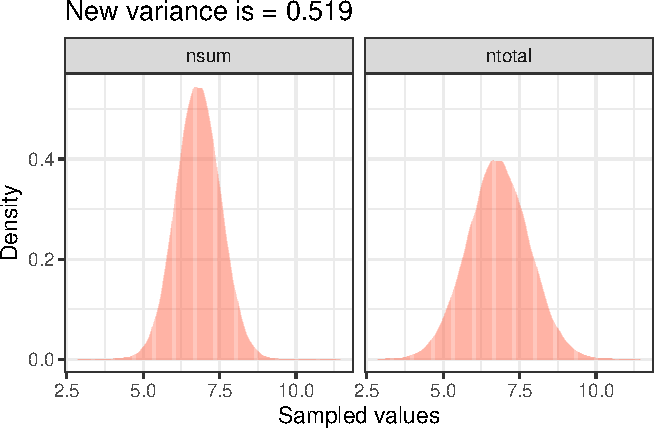
\includegraphics{exercises_files/figure-latex/unnamed-chunk-9-1} \end{center}

\begin{Shaded}
\begin{Highlighting}[]
\NormalTok{(}\FloatTok{0.6}\OperatorTok{^}\DecValTok{2}\NormalTok{)}\OperatorTok{+}\NormalTok{(}\FloatTok{0.4}\OperatorTok{^}\DecValTok{2}\NormalTok{)}
\end{Highlighting}
\end{Shaded}

\begin{verbatim}
## [1] 0.52
\end{verbatim}

\begin{Shaded}
\begin{Highlighting}[]
\KeywordTok{plot_sim}\NormalTok{(}\FloatTok{0.83}\NormalTok{);}
\end{Highlighting}
\end{Shaded}

\begin{center}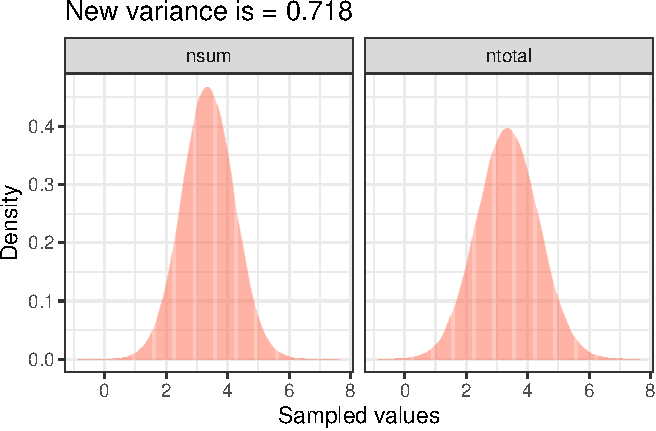
\includegraphics{exercises_files/figure-latex/unnamed-chunk-9-2} \end{center}

\begin{Shaded}
\begin{Highlighting}[]
\NormalTok{(}\FloatTok{0.83}\OperatorTok{^}\DecValTok{2}\NormalTok{)}\OperatorTok{+}\NormalTok{(}\FloatTok{0.17}\OperatorTok{^}\DecValTok{2}\NormalTok{)}
\end{Highlighting}
\end{Shaded}

\begin{verbatim}
## [1] 0.7178
\end{verbatim}

\[ log(f(\mathbf{x} | \mu, \sigma^2)) = n \thinspace log\Big(\frac{1}{\sqrt{2\pi (w^2 + (1-w)^2)}}\Big) + 
\sum_{i = 1}^{n} \frac{-(x_i - w\mu_1 - (1 - w)\mu_2)^2}{2 (w^2 + (1-w)^2)} \]

\[ 
\frac{\partial log(f(\mathbf{x} | \mu_1, \mu_2, \sigma^2))}{\partial \mu_2} \approx   
\sum_{i = 1}^{n} -(-(\mu_i - \mu_2)(-\mu_1w + x + (w - 1)\mu_2) \\
\approx   
\sum_{i = 1}^{n} (-\mu_1w + x_ + (w - 1)\mu_2)
\] \[ \hat \mu_2 = \sum_{i = 1}^{n} \frac{x_i - \mu_1w}{n(1 - w)} \]
\[ \hat \mu_1 = \sum_{i = 1}^{n} \frac{x_i - \mu_2(1-w)}{nw} \]

\textbf{Exercise A.2.} Find the estimators which minimise the posterior
expected loss for the following loss functions for continuous
parameters:

\begin{enumerate}
\def\labelenumi{(\alph{enumi})}
\tightlist
\item
  Squared-error (or quadratic) loss:
  \(C(\theta, \mathbb{V}) = (\theta - \mathbb{V})^2\).
\end{enumerate}

\[\Big[\int_{\Theta} (\theta - \mathbb{V})^2 f(\theta | x)d\theta \Big]' = -2 \int_{\Theta} (\theta - \mathbb{V}) f(\theta | x)d\theta,\]
\[-2 \int_{\Theta} (\theta - \mathbb{V}) f(\theta | x)d\theta = 0 \]
\[\mathbb{V} = \int_{\Theta} \theta  f(\theta | x)d\theta = \mathbb{E}_{\theta|x}[\theta]\]

\begin{enumerate}
\def\labelenumi{(\alph{enumi})}
\setcounter{enumi}{1}
\tightlist
\item
  Absolute-error loss:
  \(C(\theta, \mathbb{V}) = |\theta - \mathbb{V}|\).
\end{enumerate}

\[\Big[\int_{\Theta} |\theta - \mathbb{V}|f(\theta | x)d\theta \Big]' =
\Big[\int_{-\infty}^{\mathbb{V}} (-\theta + \mathbb{V})  f(\theta | x)d\theta + 
\int_{\mathbb{V}}^{\infty} (\theta - \mathbb{V}) 
f(\theta | x)d\theta \Big]'\]
\[2 \int_{-\infty}^{\mathbb{V}}f(\theta | x)d\theta =
\int_{\infty}^{\infty}f(\theta | x)d\theta = 1\\\]

and \(\mathbb{V}\) will be the median of the posterior
\(f(\theta | x)\).

and for \emph{discrete} parameters:

\begin{enumerate}
\def\labelenumi{(\alph{enumi})}
\setcounter{enumi}{2}
\tightlist
\item
  Squared-error (or quadratic) loss:
  \(C(\theta, \mathbb{V}) = (\theta - \mathbb{V})^2\).
\end{enumerate}

\[\Big[\sum^{\Theta} (\theta - \mathbb{V})^2 P(\theta | x)Big]' = -2 \sum^{\Theta}(\theta - \mathbb{V}) P(\theta | x) = 0,\]

\[\mathbb{V} = \sum^{\Theta}\theta P(\theta | x) = \mathbb{E}_{P(\theta |x)}[\theta]\]

\begin{enumerate}
\def\labelenumi{(\alph{enumi})}
\setcounter{enumi}{3}
\tightlist
\item
  Zero-one loss:
\end{enumerate}

\[
C(\theta, \mathbb{V})  = 
\begin{cases}
    0,\text{ if }\theta = \mathbb{V}, \\
    1,\text{ otherwise.} 
\end{cases}
\]

\[\sum_{\theta \in \Theta \texttt{\ } \{\theta^*\}} P(\theta | x) 
= 1 - P(\theta^* | x)\]

the \(\mathbb{V}\) will be the mode \(\theta^*\), because that is the
most likely value.

\textbf{Exercise B.1.} Given an example of a sequence of random
variables which:

\begin{enumerate}
\def\labelenumi{(\alph{enumi})}
\tightlist
\item
  converge to a limit with probability one;
\end{enumerate}

If \(X_1,\dots,X_n \sim Ber(1/2)\) and
\(Y_n = 2^n \prod_{i = 1}^n X_i\), letting \(0 < \epsilon < 2^m\),

\[
\begin{split}
 P\{|Y_n - 0| < \epsilon \text{ for all } n \geq m\} & = 
P\{X_n = 0 \text{ for some } n \leq m \} \\
& = 1 - P\{X_n = 1\text{ for all }  n \geq m \} \\
& = 1 - (1/2)^m = 1, \text{ when } n \to \infty
\end{split}
\]

\begin{enumerate}
\def\labelenumi{(\alph{enumi})}
\setcounter{enumi}{1}
\tightlist
\item
  converge to a limit in probability but not almost surely; and
\end{enumerate}

If \(X_1,\dots,X_n \sim Exp(n)\), the sequence

\[
\begin{split}
\lim_{n \to \infty} P\{|X_n - 0| \geq \epsilon \} 
& = \lim_{n \to \infty} P\{X_n \geq \epsilon\} \\
& = \lim_{n \to \infty}  e^{-n \epsilon} = 0, \text{ for all } \epsilon.
\end{split}
\]

\begin{enumerate}
\def\labelenumi{(\alph{enumi})}
\setcounter{enumi}{2}
\tightlist
\item
  converge to a limit in distribution but not in probability.
\end{enumerate}

CLT - Let \(X_1,\dots,X_n \sim U[-1, 1]\) be i.i.d. with finite mean
\(E(X)\) and some variance \(\sigma_x^2\). The normalized sum

\[ Z_n = \frac{\sum_{i = 1}^{n}X_i}{\sqrt{n/3}}\]

will quickly approach a Gaussian distribution.

\begin{Shaded}
\begin{Highlighting}[]
\NormalTok{n <-}\StringTok{ }\DecValTok{10000}
\NormalTok{unif <-}\StringTok{ }\KeywordTok{data.frame}\NormalTok{(}\DataTypeTok{unif_val =} \KeywordTok{runif}\NormalTok{(n, }\DataTypeTok{min =} \DecValTok{-1}\NormalTok{, }\DataTypeTok{max =} \DecValTok{1}\NormalTok{)) }\OperatorTok\StringTok{ }
\StringTok{  }\KeywordTok{mutate}\NormalTok{(}
    \DataTypeTok{ind =} \KeywordTok{rep}\NormalTok{(}\DecValTok{1}\NormalTok{, n), }
    \DataTypeTok{cs =} \KeywordTok{cumsum}\NormalTok{(unif_val), }
    \DataTypeTok{ns =} \KeywordTok{cumsum}\NormalTok{(ind),}
    \DataTypeTok{zn =}\NormalTok{ cs}\OperatorTok{/}\NormalTok{(}\KeywordTok{sqrt}\NormalTok{(ns}\OperatorTok{/}\DecValTok{3}\NormalTok{)))}

\NormalTok{unif }\OperatorTok\StringTok{ }
\StringTok{  }\KeywordTok{ggplot}\NormalTok{(}\KeywordTok{aes}\NormalTok{(zn, }\KeywordTok{dnorm}\NormalTok{(zn))) }\OperatorTok{+}
\StringTok{  }\KeywordTok{geom_line}\NormalTok{(}\DataTypeTok{colour =} \StringTok{"tomato"}\NormalTok{, }\DataTypeTok{alpha =} \FloatTok{0.3}\NormalTok{, }\DataTypeTok{size =} \DecValTok{2}\NormalTok{) }\OperatorTok{+}
\StringTok{  }\KeywordTok{stat_function}\NormalTok{(}\DataTypeTok{fun =}\NormalTok{ dnorm, }\DataTypeTok{args =} \KeywordTok{list}\NormalTok{(}\DataTypeTok{mean =} \DecValTok{0}\NormalTok{, }\DecValTok{1}\NormalTok{), }
                \DataTypeTok{linetype =} \DecValTok{3}\NormalTok{)}\OperatorTok{+}
\StringTok{  }\KeywordTok{xlim}\NormalTok{(}\OperatorTok{-}\FloatTok{2.5}\NormalTok{, }\FloatTok{2.5}\NormalTok{) }\OperatorTok{+}\StringTok{ }
\StringTok{  }\KeywordTok{theme_bw}\NormalTok{()}
\end{Highlighting}
\end{Shaded}

\begin{center}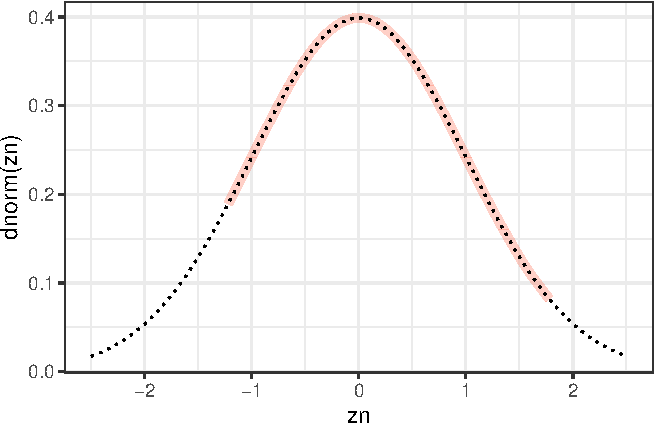
\includegraphics{exercises_files/figure-latex/unnamed-chunk-10-1} \end{center}


\end{document}
